\documentclass[tikz,border=2pt]{standalone}
\usepackage{amsmath}
\usepackage{pgfplots}
\pgfplotsset{compat=1.18}
\usetikzlibrary{arrows.meta}
\begin{document}
% Arrival counts a_1..a_10 = 8,12,9,11,10,7,13,10,9,11 per period: mean 10, (1/n) sum a_i^2 - mean^2 = 3,
% so C_a^2 is estimated by 3/10 = 0.3.
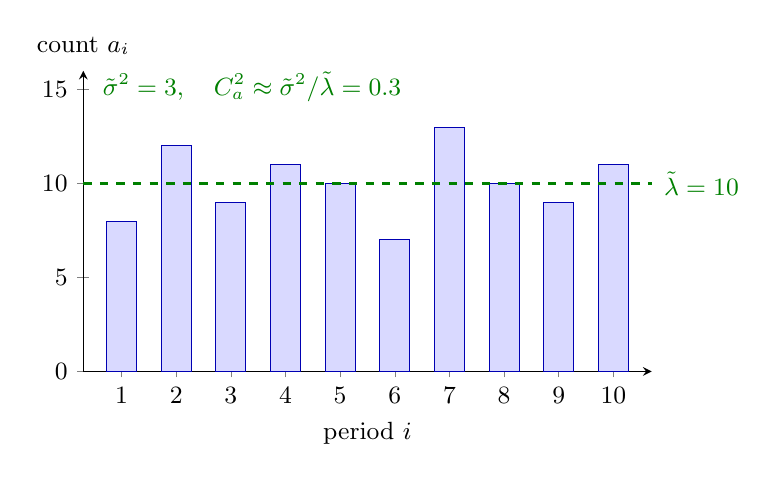
\begin{tikzpicture}[font=\small, >={Latex[length=2mm]}]
  \begin{axis}[
    axis lines=left, xmin=0.3, xmax=10.7, ymin=0, ymax=16,
    xtick={1,...,10}, ytick={0,5,10,15},
    xlabel={period $i$}, ylabel={count $a_i$},
    ylabel style={rotate=-90, anchor=south, at={(axis description cs:0,1.02)}},
    width=8.8cm, height=5.4cm, clip=false]
    \addplot[ybar, bar width=0.55, draw=blue!70!black, fill=blue!15] coordinates
      {(1,8) (2,12) (3,9) (4,11) (5,10) (6,7) (7,13) (8,10) (9,9) (10,11)};
    \draw[green!50!black, very thick, dashed] (axis cs:0.3,10) -- (axis cs:10.7,10);
    \node[green!50!black, anchor=west] at (axis cs:10.75,10) {$\tilde{\lambda}=10$};
    \node[green!50!black, anchor=south west, fill=white, inner sep=1pt] at (axis cs:0.6,14.2) {$\tilde{\sigma}^2=3,\quad C_a^2\approx\tilde{\sigma}^2/\tilde{\lambda}=0.3$};
  \end{axis}
\end{tikzpicture}
\end{document}
